\documentclass[tikz,border=6pt]{standalone}
\usepackage[T1]{fontenc}
\usepackage[utf8]{inputenc}
\usepackage{amsmath,amssymb}
\usepackage{tikz}
\usetikzlibrary{automata,positioning,arrows.meta,shapes.geometric,calc,fit}
\tikzset{
    >=Stealth,
    every state/.style={minimum size=8mm, inner sep=1pt, font=\small},
    flow/.style={rectangle, rounded corners, draw, align=center, minimum width=3.1cm, minimum height=0.9cm},
    decision/.style={diamond, draw, aspect=2.0, align=center, inner sep=1.5pt},
    terminal/.style={ellipse, draw, align=center, minimum width=2.4cm, minimum height=0.85cm},
    module/.style={rectangle, draw, rounded corners, align=center, minimum width=3.4cm, minimum height=1.0cm},
    data/.style={rectangle, draw, align=center, minimum width=3.2cm, minimum height=0.9cm}
}
\begin{document}
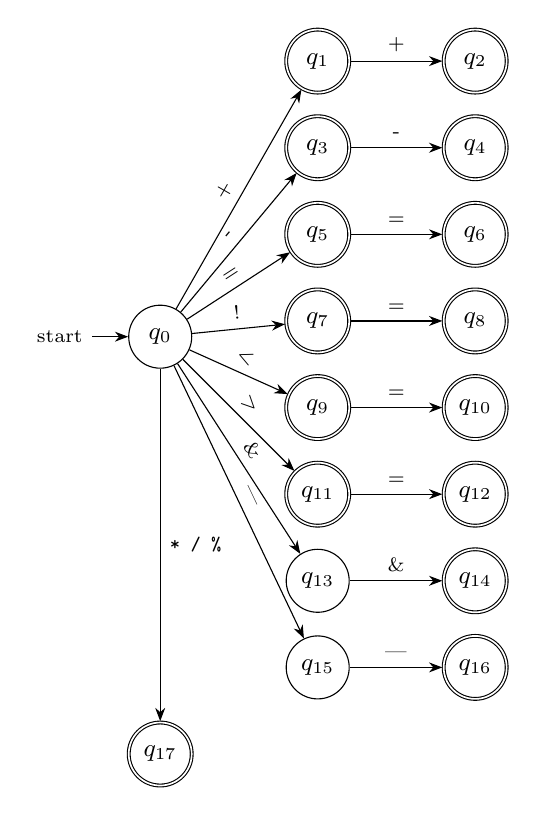
\begin{tikzpicture}[->, font=\scriptsize]
    \node[state, initial] (q0) at (0,0) {$q_0$};

    \node[state, accepting] (plus)  at (2,3.5) {$q_1$};
    \node[state, accepting] (plusplus) at (4,3.5) {$q_2$};
    \path (q0) edge node[above,sloped] {+} (plus)
          (plus) edge node[above] {+} (plusplus);

    \node[state, accepting] (minus) at (2,2.4) {$q_3$};
    \node[state, accepting] (minusminus) at (4,2.4) {$q_4$};
    \path (q0) edge node[above,sloped] {-} (minus)
          (minus) edge node[above] {-} (minusminus);

    \node[state, accepting] (eq) at (2,1.3) {$q_5$};
    \node[state, accepting] (eqeq) at (4,1.3) {$q_6$};
    \path (q0) edge node[above,sloped] {=} (eq)
          (eq) edge node[above] {=} (eqeq);

    \node[state, accepting] (not) at (2,0.2) {$q_7$};
    \node[state, accepting] (noteq) at (4,0.2) {$q_8$};
    \path (q0) edge node[above,sloped] {!} (not)
          (not) edge node[above] {=} (noteq);

    \node[state, accepting] (less) at (2,-0.9) {$q_9$};
    \node[state, accepting] (lesseq) at (4,-0.9) {$q_{10}$};
    \path (q0) edge node[above,sloped] {$<$} (less)
          (less) edge node[above] {=} (lesseq);

    \node[state, accepting] (greater) at (2,-2.0) {$q_{11}$};
    \node[state, accepting] (greatereq) at (4,-2.0) {$q_{12}$};
    \path (q0) edge node[above,sloped] {$>$} (greater)
          (greater) edge node[above] {=} (greatereq);

    \node[state] (and1) at (2,-3.1) {$q_{13}$};
    \node[state, accepting] (and2) at (4,-3.1) {$q_{14}$};
    \path (q0) edge node[above,sloped] {\&} (and1)
          (and1) edge node[above] {\&} (and2);

    \node[state] (or1) at (2,-4.2) {$q_{15}$};
    \node[state, accepting] (or2) at (4,-4.2) {$q_{16}$};
    \path (q0) edge node[above,sloped] {|} (or1)
          (or1) edge node[above] {|} (or2);

    \node[state, accepting] (single) at (0,-5.3) {$q_{17}$};
    \path (q0) edge node[right] {\texttt{* / \%}} (single);
\end{tikzpicture}
\end{document}
